\chapter{Sherbrooke}\label{ch:ch3label}

Ce chapitre est exclusivement dédié aux bidiplômes pour Sherbrooke. La particularité de ce bidiplôme est qu’il n’y a aucun test à passer au préalable. Seul le dossier est à envoyer et tout est gratuit (concernant la demande d’admission du moins). C’est donc une bonne solution de «replie» lorsque l’on veut absolument partir. Le point fort du bidiplôme à Sherbrooke est qu’il peut être diplômant suivant les cours que l’on choisit et il est très loin d’être aussi cher que Chicago ou Audencia par exemple. Un bidiplôme n’est pas forcément excessif en termes de prix et peut vous apporter une plus-value non négligeable sur votre CV, mais surtout sur votre expérience personnelle.

\section{Les bidiplômes proposés}\label{sec:sec3.1}

Plusieurs options s'offrent à vous pour cette destination comme le génie électrique ou informatique, mais aussi le bidiplôme informatique orienté jeux vidéo sponsorisé par Ubisoft. Il peut se faire en un ou deux ans et est diplômant avec un stage de fin d'études de 6 mois obligatoire. Je parle d'un ou deux ans, car c'est possible d'avoir les 45 crédits ECTS demandé par l'ESEO en un an (15 crédits par session), mais si vous suivre plus de deux cours techniques (les séries 700 expliquées plus tard) cela devient tout de même compliqué. Mais loin d'être infaisable! Sinon vous pouvez le faire un an et un trimètre en plus pour compléter vos crédits.
Je vous renvoie aussi vers la section \ref{sec:sec3.2.9} [link] qui précisera le choix des cours et la section \ref{sec:sec4.7.1} [link] pour leurs déroulements. Cela éclaircira grandement le grand flou à ce sujet.


\section{L'administratif}\label{sec:sec3.2}
L'administratif n'est pas si terrible que cela non plus, mais veillez à vous y prendre longtemps à l'avance. Au moment où je vous écris ce document, nous sommes le 20 août et j'ai finalement tous les documents me permettant de partir. J’ai quand même reçu mon permis d’étude, dernières pièces du puzzle 5 jours avant mon départ... J’étais laaaaaaarge. Les règles d’or sont donc:
\begin{description}
  \item[$\bullet$]Toujours faire tout dé que possible.
  \item[$\bullet$]Si vous avez un problème quelconque, demandé! Bombardé de mails, d'appel ou autre.
  \item[$\bullet$]Ne demander pas à l'ESEO. Déjà par pure incompétence du service, mais surtout parce qu'ils s'en foutent royalement.
  \item[$\bullet$]Restez attentifs aux mises à jour de statuts et à votre adresse postale!
  En effet, c’est souvent le moment de lâcher un appartement, n’oubliez pas donc de mettre une adresse fixe, ou si vous n’en avez pas comme ça a été le cas pour moi, la poste peut vous mettre à disposition une boîte postale, ou une redirection du courrier.
  \item[$\bullet$]Dernière règle et pas des moindres, numérisé et conservé plusieurs copies de vos documents originaux! Beaucoup de documents à fournir sont identiques pour certaines démarches, cela vous conserve du temps, et surtout si vous devez en renvoyer un en urgence, vous pouvez le faire sans problèmes!
\end{description}

\bigbreak
\href{https://www.usherbrooke.ca/etudiants-internationaux/fr/guide-daccueil/avant-votre-arrivee/papiers-legaux/}{\textbf{Page de l'UdeS rassemblant les principaux papiers administratif à fournir}}\textsubscript{  [link]}

\subsection{La procédure d'incription}\label{sec:sec3.2.1}
Je vous épargne un long discours et vous montrez ces deux diagrammes. La timeline de la procédure dans un premier temps qui vous permettra de prévoir sereinement votre procédure d'inscription. Le deuxième diagramme disponible dans section \ref{sec:sec3.2.10} [link] montre les différents procédures et documents à fournir. Le nombre d'acteurs engagés est important, mais beaucoup se font très simplement et facilitent grandement votre entrée sur le territoire Québécois. Je pense notamment au VAE et à Accueil Plus ou seul un document en ligne est à remplir.
En revanche, il est important de porter une attention particulière au CAQ. C'est un document vital pour votre entrée sur le territoire et le permis d'étude en dépend directement! (i.e. pas de CAQ pas de permis d'étude, pas de permis d'étude pas d'université, pas d'université pas de diplôme, pas de diplôme = finir ses jours à l'ESEO.)

\begin{figure}[h!]
\centering
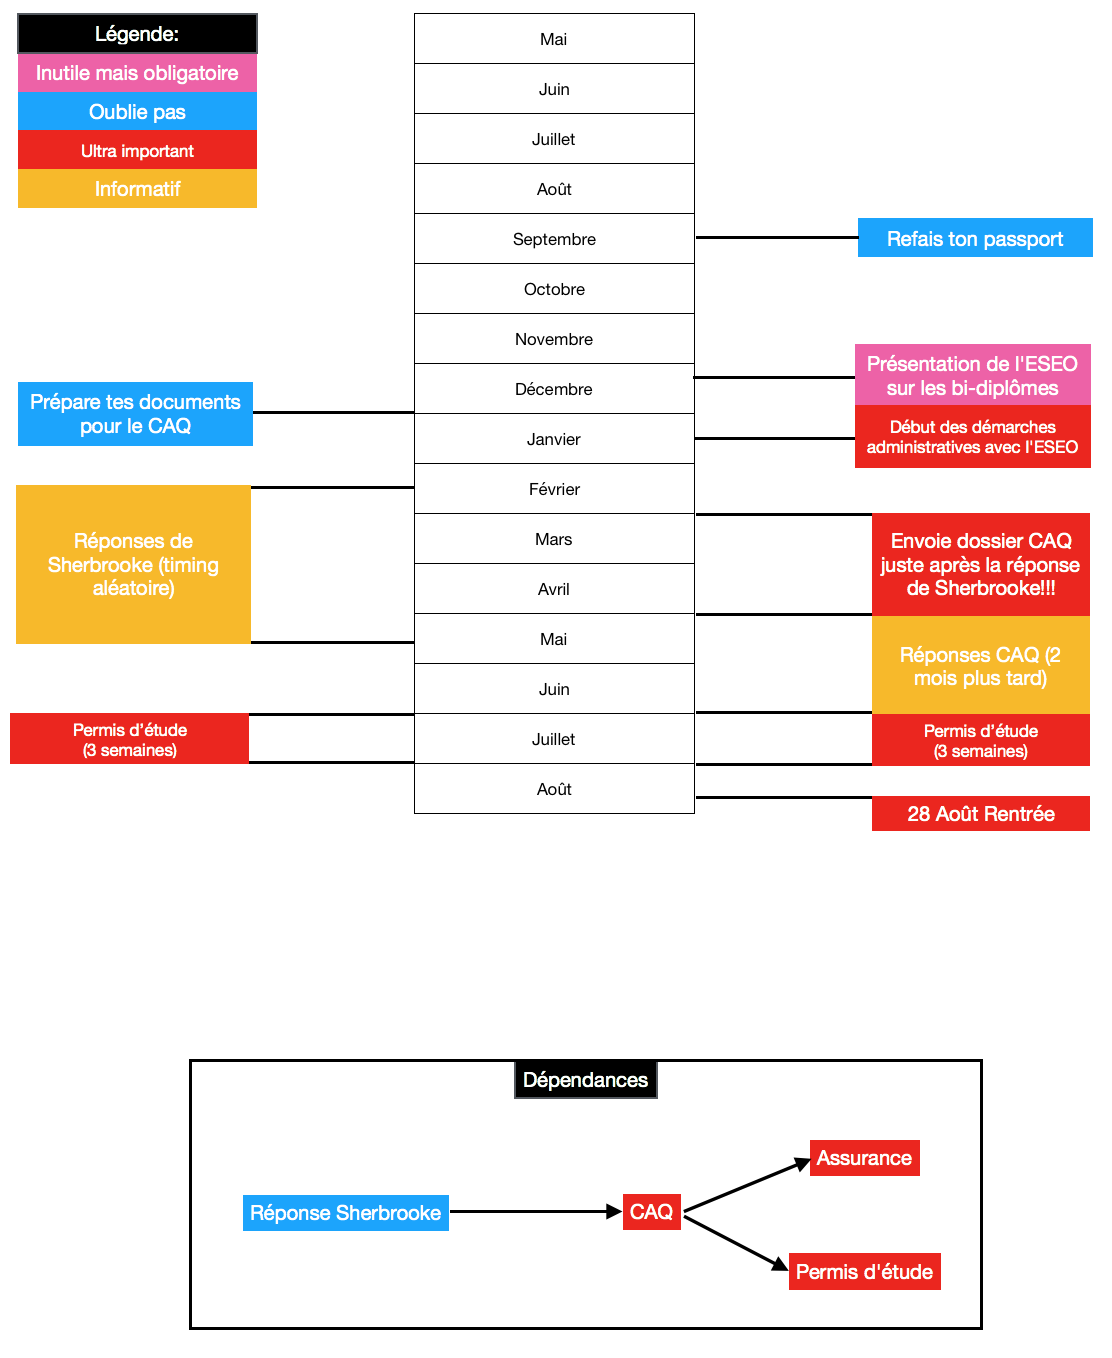
\includegraphics[width = 90mm]{figures/Chrono_Sherbrooke}
\caption{Frise chronologique approximative des différentes étapes administratives}
\end{figure}

\subsection{Inscription à l'université}\label{sec:sec3.2.2}
Après avoir mentionné au près de l'ESEO que vous vouliez partir d'ici, je vous invite à vous rendre sur le site suivant pour commencer la procédure: \\
\href{https://www.usherbrooke.ca/helios/lib880/infoadm/cw/wda1/CLW301F1}{\textbf{Lien vers la page d'inscription de l'UdeS}}\textsubscript{  [link]}


\begin{example}{L'incompétence à l'état pur}
  Pour la petite histoire, la personne "en charge" des bidiplôme n'a aucune idée du lien pour l'inscription. C'est un élève qui a du envoyer un bon nombres d'emails à l'UdeS pour avoir ce lien... Quand je vous dis que vous êtes seul en voici un petit exemple.
\end{example}


\subsection{Les joies du CAQ}\label{sec:sec3.2.3}
Qu'est-ce que le CAQ? C'est le Certificat d'Acceptation du Québec, en gros votre visa étudiant. Cela sera le papier le plus long à obtenir!
Voilà tous les papiers à fournir une fois votre demande en ligne passée et payée. Certains documents mettre du temps à être obtenu surtout les documents bancaires, veillez donc à vous y prendre à l'avance. \\
Cela se fait à travers le site du ministère:
\bigbreak
\href{http://www.immigration-quebec.gouv.qc.ca/fr/services/caq-electronique/index.html}{\textbf{Page de connexion au compte de CAQ}}\textsubscript{  [link]}
\bigbreak
Descendez en fin de page pour vous y inscrire ou même pour consulter votre dossier.

\begin{figure}[h!]
\centering
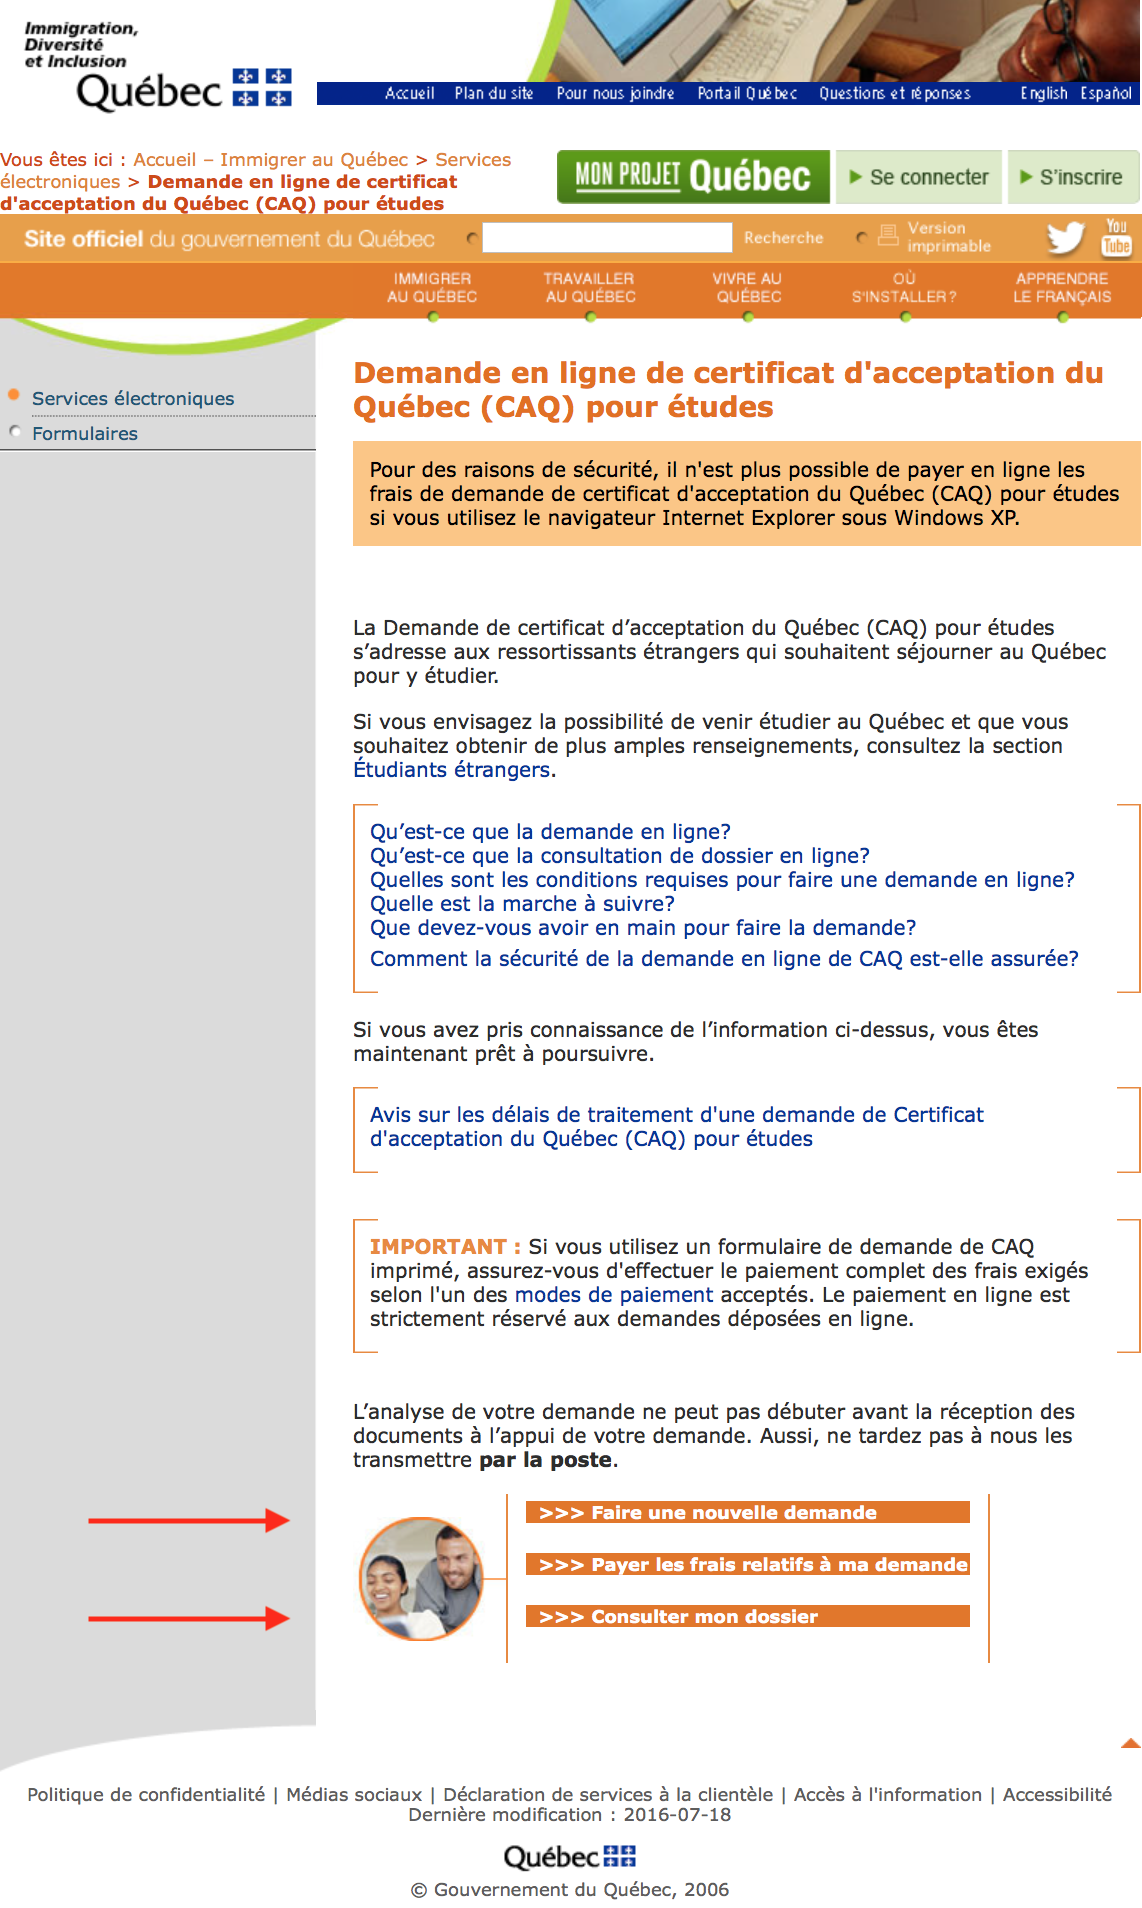
\includegraphics[width = 80mm]{figures/Site_CAQ}
\caption{Voici à quoi la page internet devrait ressembler}
\end{figure}


\begin{example}{Les délais de traitement}
  Le ministère canadien se donne six semaines à partir de la réception des documents pour traiter votre demande. Cela peu aller plus vite, mais c’est rare. Vous n’aurez aucune donnée ou confirmation de réception tant que la demande n’est pas en cours de traitement! Veillez donc bien à prendre un vos dispositions la dessus.
  IMPORTANT: Par expérience, je vous déconseille la poste! Ils mettront 1 mois de traitement pour votre demande et bien que vous allez payer un recommandé avec accusé de réception, cette accusée ne sera jamais renvoyée, car le Canada ne connaît pas cela pour la poste.
  Je vous conseille donc DHL, UPS ou tout autre livreur privé qui vous garantira une réception du plie avec accusé de réception en moins d’une semaine pour un prix avoisinant les 80\euro{}. Je vous le conseille fortement, cela vous évitera de gros problèmes par la suite, car tout autre document dépend directement du CAQ!
  J’insiste sur cette partie, car elle est primordiale dans vos démarches, après c’est un jeu d’enfant.
\end{example}

\subsection{Demande de dérogation}\label{sec:sec3.2.4}
La demande de dérogation doit s'effectuer avant le 30 juin de l'année où vous partez de l'ESEO. Oui, il faut que l'on décide de ne pas revenir avant même d'être parti! C'est l'une des nombreuses informations que l'on vous donne juste avant votre départ quand tout est bouclé... Je vous laisse voir cela avec votre directeur des études actuel, B. Haussy pour savoir si vous avez tout bien validé et qu'il donne son accord que vous vous détachiez définitivement de cette école.
\bigbreak
\href{Annexes/Sherbrooke/Demande_Derogation_COSNEAU_Alexandre.pdf}{\textbf{Exemple de lettre de dérogation}}\textsubscript{  [link]}

\subsection{Bourse ENVOLEO}\label{sec:sec3.2.5}
La bourse ENVOLEO est accessible, pour n'importe quel élève partant à l'étranger peu importe le revenu des parents. Elle est d'approximativement 1272\$ CA si mes souvenirs sont bons. Et c'est à partir du mois de juin que la personne "en charge des bidiplômes" de l'ESEO vous donnera le code de l'établissement pour que vous puissiez vous inscrire sur leur site ENVOLEO. Je ne peux pas vous en dire plus là-dessus pour le moment, nous sommes le 3 octobre 2017 lorsque je vous écris et je n'ai toujours aucun retour là-dessus...

\bigbreak
\href{http://www.envoleo.paysdelaloire.fr}{\textbf{Page de connexion à la bourse ENVOLEO}}\textsubscript{  [link]}
\bigbreak

\begin{figure}[h!]
\centering
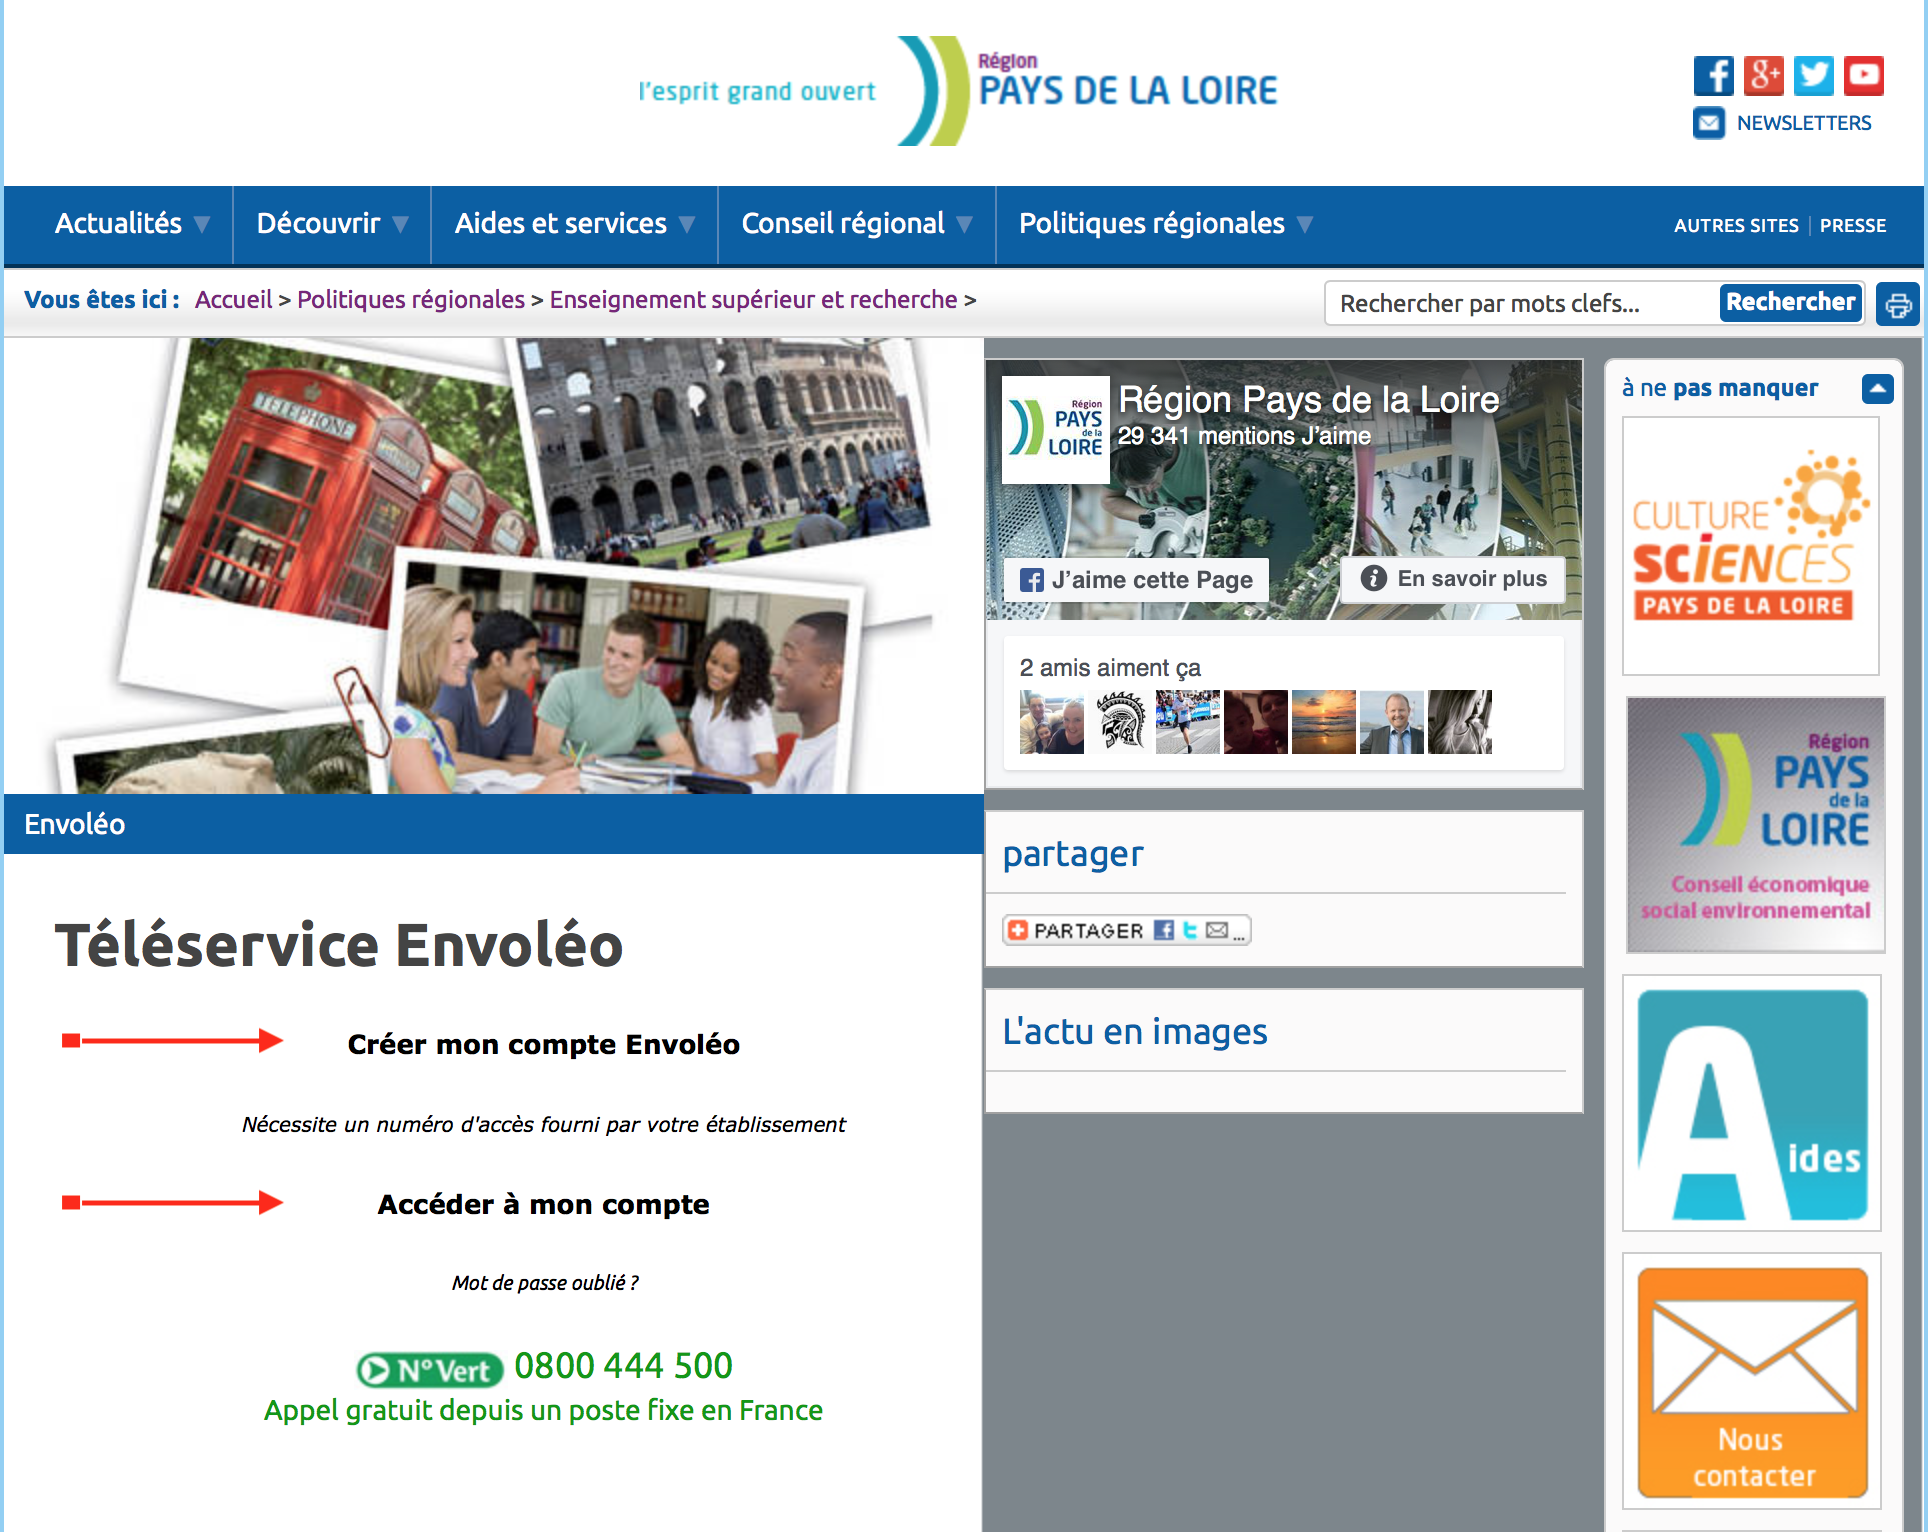
\includegraphics[width = 80mm]{figures/Site_Envoleo}
\caption{Voici à quoi la page internet devrait ressembler}
\end{figure}


\subsection{Le permis d'étude}\label{sec:sec3.2.6}
Directement après avoir reçu votre CAQ par mail, je vous conseille de commencer vos démarches pour le permis d'étude. Même si celui-ci met au maximum 2 semaines pour être validé, c'est toujours mieux de s'y prendre à l'avance.

\begin{figure}[h!]
\centering
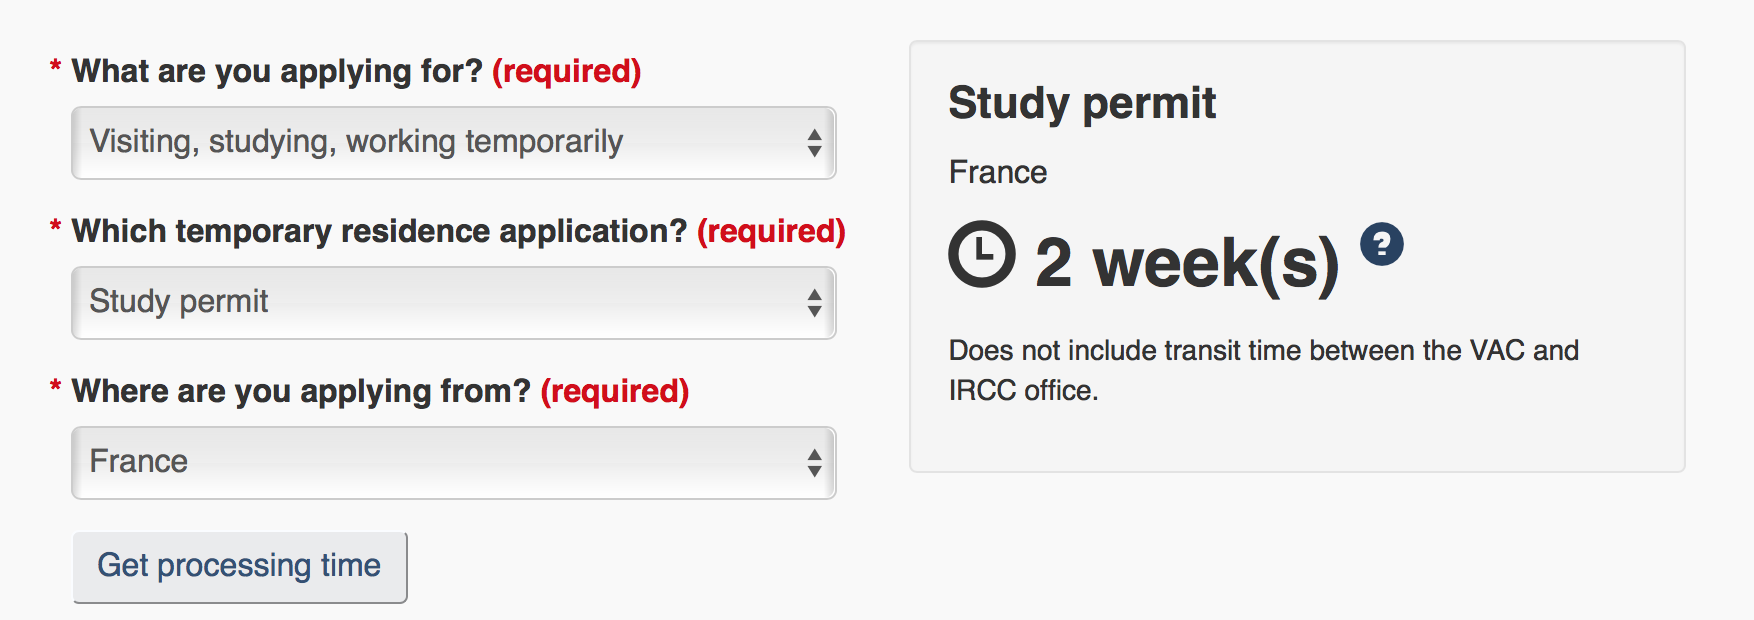
\includegraphics[width = 80mm]{figures/Processing_Time_SP}
\caption{Temps d'attente pour le permis d'étude}
\end{figure}

Tout se fait à travers ce site:
\bigbreak
\href{http://www.cic.gc.ca/francais/services-e/compte.asp}{\textbf{Page de connexion au permis d'étude}}\textsubscript{  [link]}
\bigbreak

\begin{example}{Des petits trucs à savoir}
  Utilisez l'option CléGc pour vous connecter au site.
  Contrairement au CAQ, tout se fait sur le site ce qui est accélère grandement la demande. \\
  Pour le document IMM1294, ne le téléchargez pas. cela vous donnera un document illisible. \\
  Il faudra l'ouvrir dans un nouvel onglet sur Google Chrome, car il se préremplit directement. \\
  \textbf{Pour la délivrance finale du permis d'étude, cela se fera à la douane canadienne.}
\end{example}

\begin{figure}[h!]
\centering
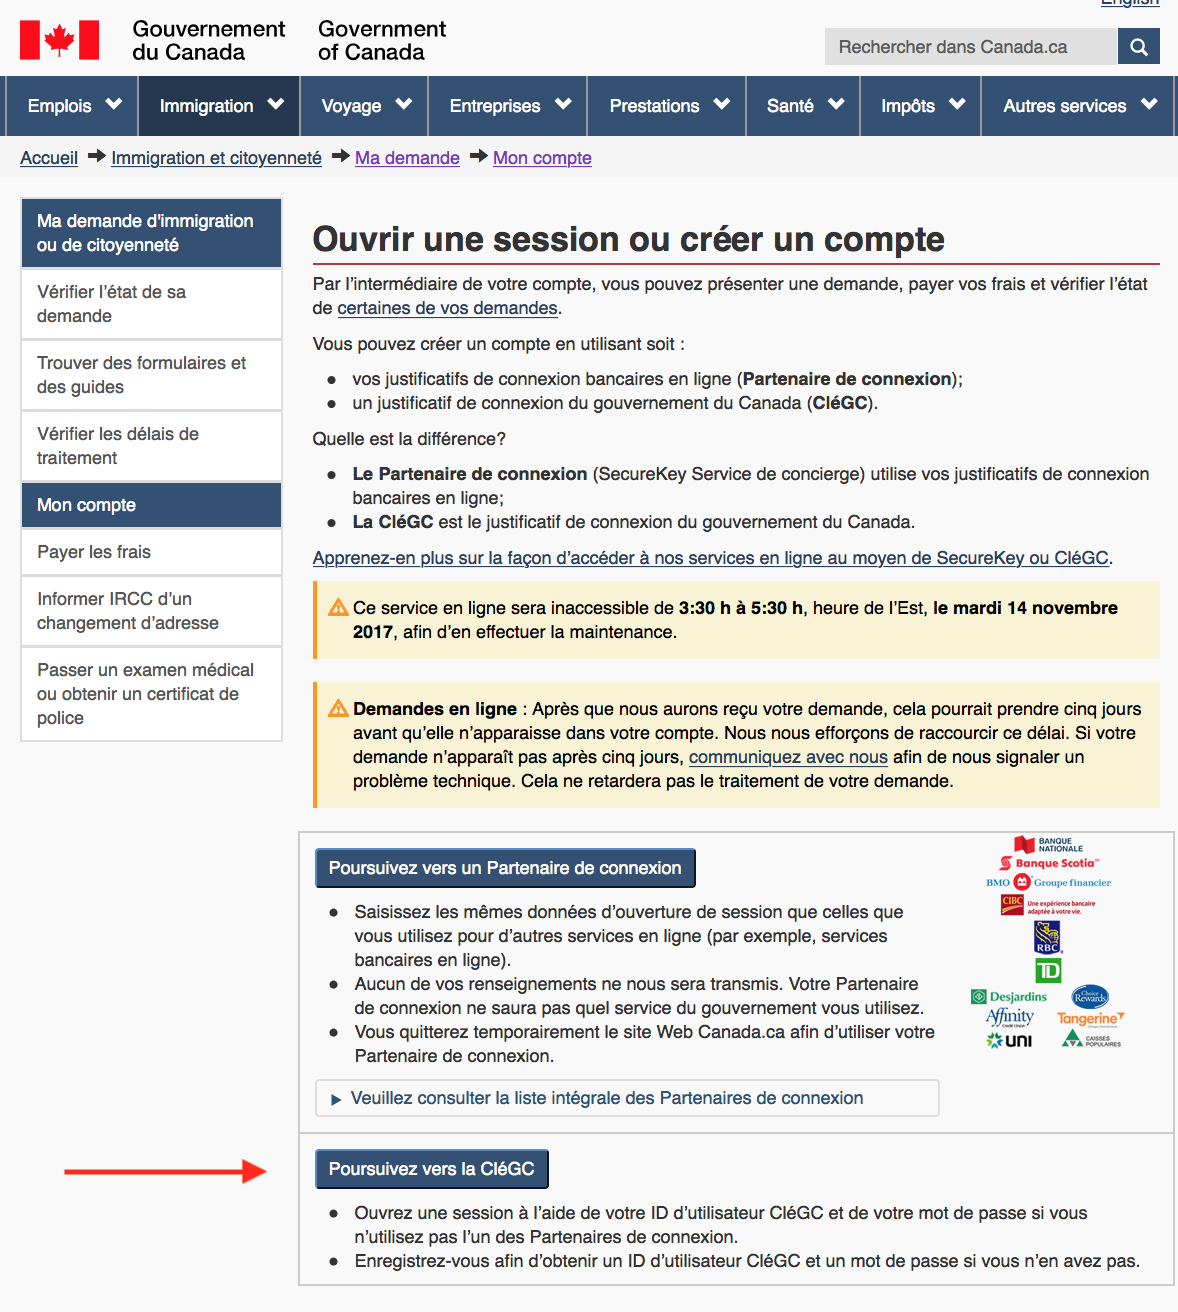
\includegraphics[width = 80mm]{figures/Site_Permis_Etude}
\caption{Voici à quoi la page internet devrait ressembler}
\end{figure}


\begin{example}{Les documents pour la douane}
 Ce qu'il vous faut impérativement à la douane Canadienne:
 \begin{description}
   \item[$\bullet$]Toujours faire tout dé que possible.
   \item[$\bullet$]Si vous avez un problème quelconque, demandez! Bombardez de mails, d’appelez ou autre.
   \item[$\bullet$]Ne demander pas à l’ESEO. Déjà par pure incompétence du service, mais surtout parce qu’ils s’en foutent royalement.
   \item[$\bullet$]Restez attentifs aux mises à jour de statuts et à votre adresse postale!
   En effet c’est souvent le moment de lâcher un appartement, n’oubliez pas donc de mettre une adresse fixe, ou si vous n’en avez pas comme ça a été le cas pour moi, la poste peut vous mettre à disposition une boîte postale, ou une redirection du courrier.
   \item[$\bullet$]Dernière règle et pas des moindres, numérisez et conservez plusieurs copies de vos documents originaux! Beaucoup de documents à fournir sont identiques pour certaines démarches, cela vous fera gagner du temps, et surtout si vous devez en renvoyer un en urgence...
 \end{description}
\end{example}


 \subsection{Les assurances}\label{sec:sec3.2.7}
 Une assurance est obligatoire pour partir là-bas et c'est un motif de retour aux frontières si vous y allez sans. Prenez donc vos précautions pour cela, la SMEBA fait généralement une intervention à l'ESEO pour cela, allez-y. La particularité du Québec est que notre sécurité sociale française et celle québécoise s'associent pour faciliter les démarchent. Pour se faire, il vous faut faire signer par votre PCAM où vous êtes rattaché ce document:

 \bigbreak
 \href{Annexes/Sherbrooke/SE401-Q-102.pdf}{\textbf{Formulaire SE401-Q-102}\footnote{Le document à pu changer entre temps, prenez soin de vérifier sa validité au près de votre CPAM}}\textsubscript{  [link]}
 \bigbreak


 Cela prend 10 jours (10 jours pour l'administration française c'est 20 jours pour le reste du monde) à faire! Ne traînez donc pas.
 À cela il faut ajouter une complémentaire, c'est là que la SMEBA rentre en jeux. Pour cela, un simple coup de fil est nécessaire, c'est rapide et vous recevrez votre carte d'assurance par la poste dans les jours suivants.


 \begin{example}{Le délai est trop sérré?}
   Si vraiment le délai est trop serré pour vous, i.e. que vous devez prendre votre avion la semaine prochaine et que vous n'avez toujours rien commencé, vous pouvez envoyer un mail comme celui-ci:
   Pour Thomas EVENAT et moi, cela a marché et nous avons eu ce document en 3 jours.
 \end{example}

 \begin{figure}[h!]
 \centering
 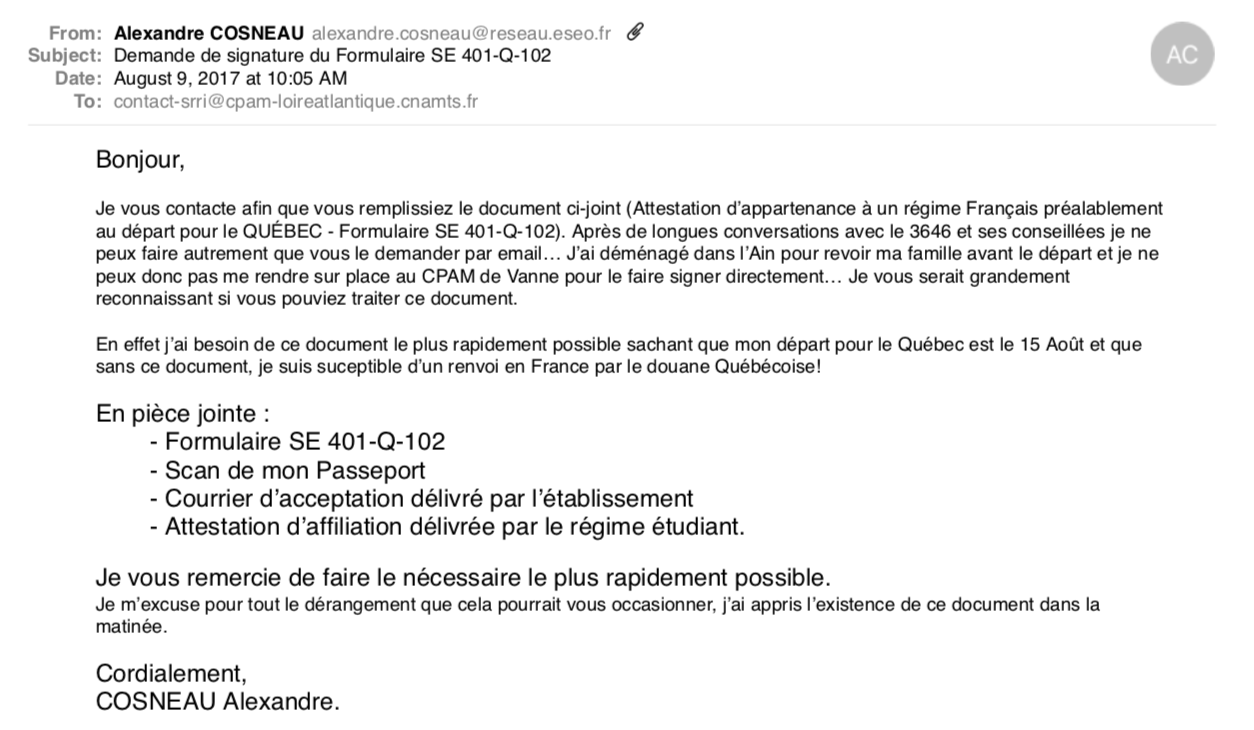
\includegraphics[width = 80mm]{figures/Mail_CPAM}
 \caption{Exemple de mail pour la signature du formulaire au près de la CPAM}
 \end{figure}

 \subsection{Accueil Plus}\label{sec:sec3.2.8}
 Accueil plus est très utile, il vous permet d'être accueilli bien plus rapidement par la douane canadienne avec de l'aide en plus. Mais surtout, c'est le plus simple à faire! 5 minutes sur leur site et le tour est joué, vous avez la réponse par mail dans les heures qui suivent!
 Les documents demandés sont le numéro de vol, le numéro de passeport, de CAQ et de permis d’étude, ce que vous devriez avoir depuis le temps.
 Faites-le vraiment.

\bigbreak
\href{http://www.accueilplus.ca/}{\textbf{URL du site d'Accueil Plus}}\textsubscript{  [link]}


\subsection{Choix des cours}\label{sec:sec3.2.9}

Début août, vous allez recevoir un mail comme celui-ci:

\bigbreak
\href{Annexes/Sherbrooke/Mail_Info_UdeS.pdf}{\textbf{Mail d'information de l'UdeS}}\textsubscript{  [link]}
\bigbreak

Vous demandant de commencer les démarches administratives pour l'université cette fois-ci. Cela inclut le choix des cours, la mise en place de votre adresse mail et de vos accès au portail, etc.
\bigbreak
\textbf{C'est le mail le plus important que vous allez recevoir de l'UdeS. Lisez le bien, il contient les informations sur vos présentation de cours (où vous devez impérativement être présent) et bien d'autres informations encore!}

\bigbreak
\href{https://www.usherbrooke.ca/helios/lib880/dosetu/menu_offert.htm}{\textbf{Lien vers votre dossier étudiant}}\textsubscript{  [link]}
\bigbreak

 La liste des cours est longue et variée, cependant \textbf{tout vous sera expliqué sur place.} Vous allez avoir une présentation faite par votre responsable d’études qui vous expliquera et vous suivra ensuite individuellement sur votre parcours. Ne paniquez pas donc faites un choix de cours bidons au début, vous avez jusqu'à début \textbf{15 septembre} pour changer votre choix.

 \bigbreak
 \href{Annexes/Sherbrooke/Date_Limite.pdf}{\textbf{Dates butoires d'inscription ou d'abandon de cours}}\textsubscript{  [link]}
 \bigbreak

\bigbreak
\href{Annexes/Sherbrooke/Annuaire_Genie_Electrique.pdf}{\textbf{Annuaire des cours de génies de l'UdeS}}\textsubscript{  [link]}
\bigbreak

\href{https://www.usherbrooke.ca/admission/programme/620/maitrise-en-genie-electrique/}{\textbf{Je vous laisse ce lien qui est un bon point de départ pour connaitre un peu l'organisation des cours à l'UdeS}}\textsubscript{  [link]}
\bigbreak

Je vous montre un exemple, c'est approximativement le mon parcous choisi a l'UdeS, ça vaudra surement mieux qu'un long discours, voici comment pourrais se dérouler votre année.

\begin{figure}[h!]
\centering
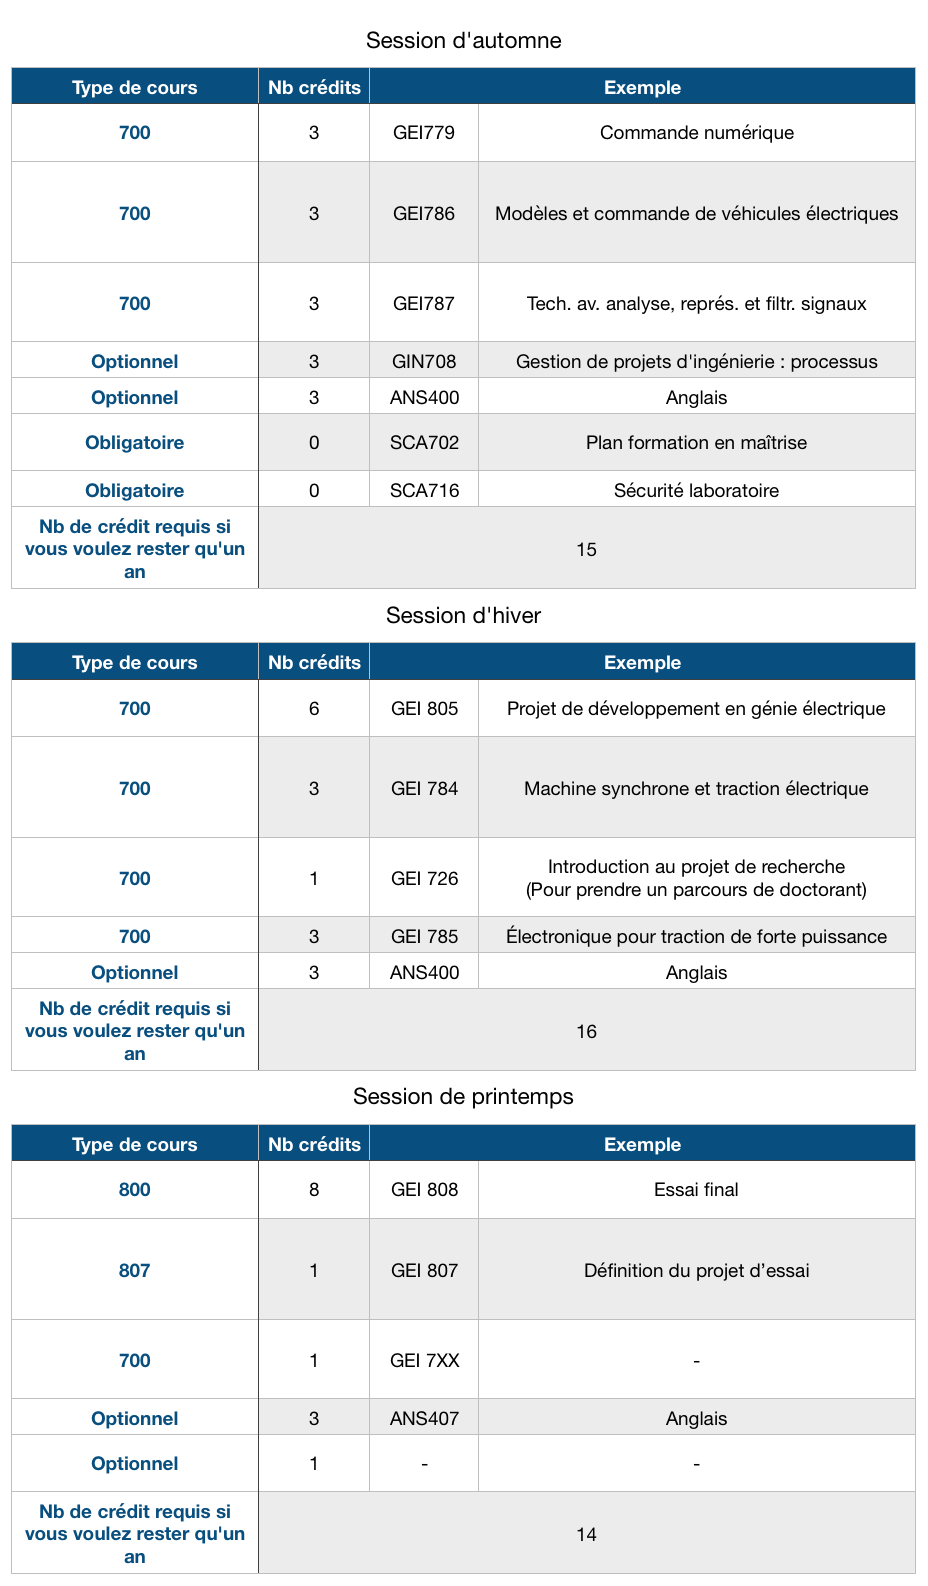
\includegraphics[width = 130mm]{figures/Exemple_Sess}
\caption{Exemple de choix de cours à l'UdeS}
\end{figure}
\clearpage


 \subsection{Récapitulons}\label{sec:sec3.2.10}
 Voici le récaitulatif des documents à obtenir pour avoir le droit de partir.
 \begin{description}
   \item[$\bullet$]Acceptation de l'Université de Sherbrooke.
   \item[$\bullet$]Passport renouvelé ou assez récent.
   \item[$\bullet$]Certificat médicale si soin permanent. (optionnel)
   \item[$\bullet$]Bourse pour une aide financière.
   \item[$\bullet$]Demande de dérogation si tu ne veux pas revenir (optionnel)
   \item[$\bullet$]CAQ.
   \item[$\bullet$]Permis d'étude.
   \item[$\bullet$]Choix des cours et débuts administratif pour l'université.
   \item[$\bullet$]VAE (compris dans le permis d'étude donc optionnel)
   \item[$\bullet$]Accueil Plus.
   \item[$\bullet$]Assurances.
 \end{description}

 \begin{figure}[h!]
 \centering
 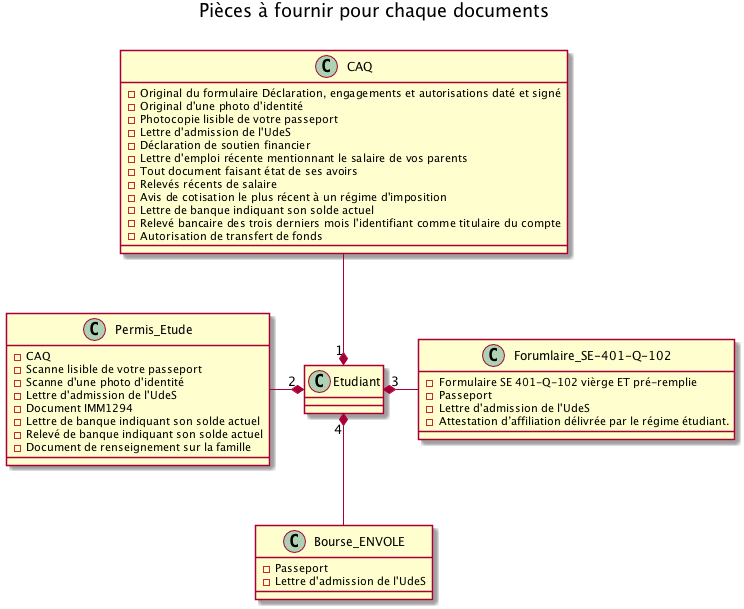
\includegraphics[width = 120mm]{figures/Documents_Demandeplantuml}
 \caption{Récapitulatif des documents à fournir pour chaque papier}
 \end{figure}

 \begin{figure}[h!]
 \centering
 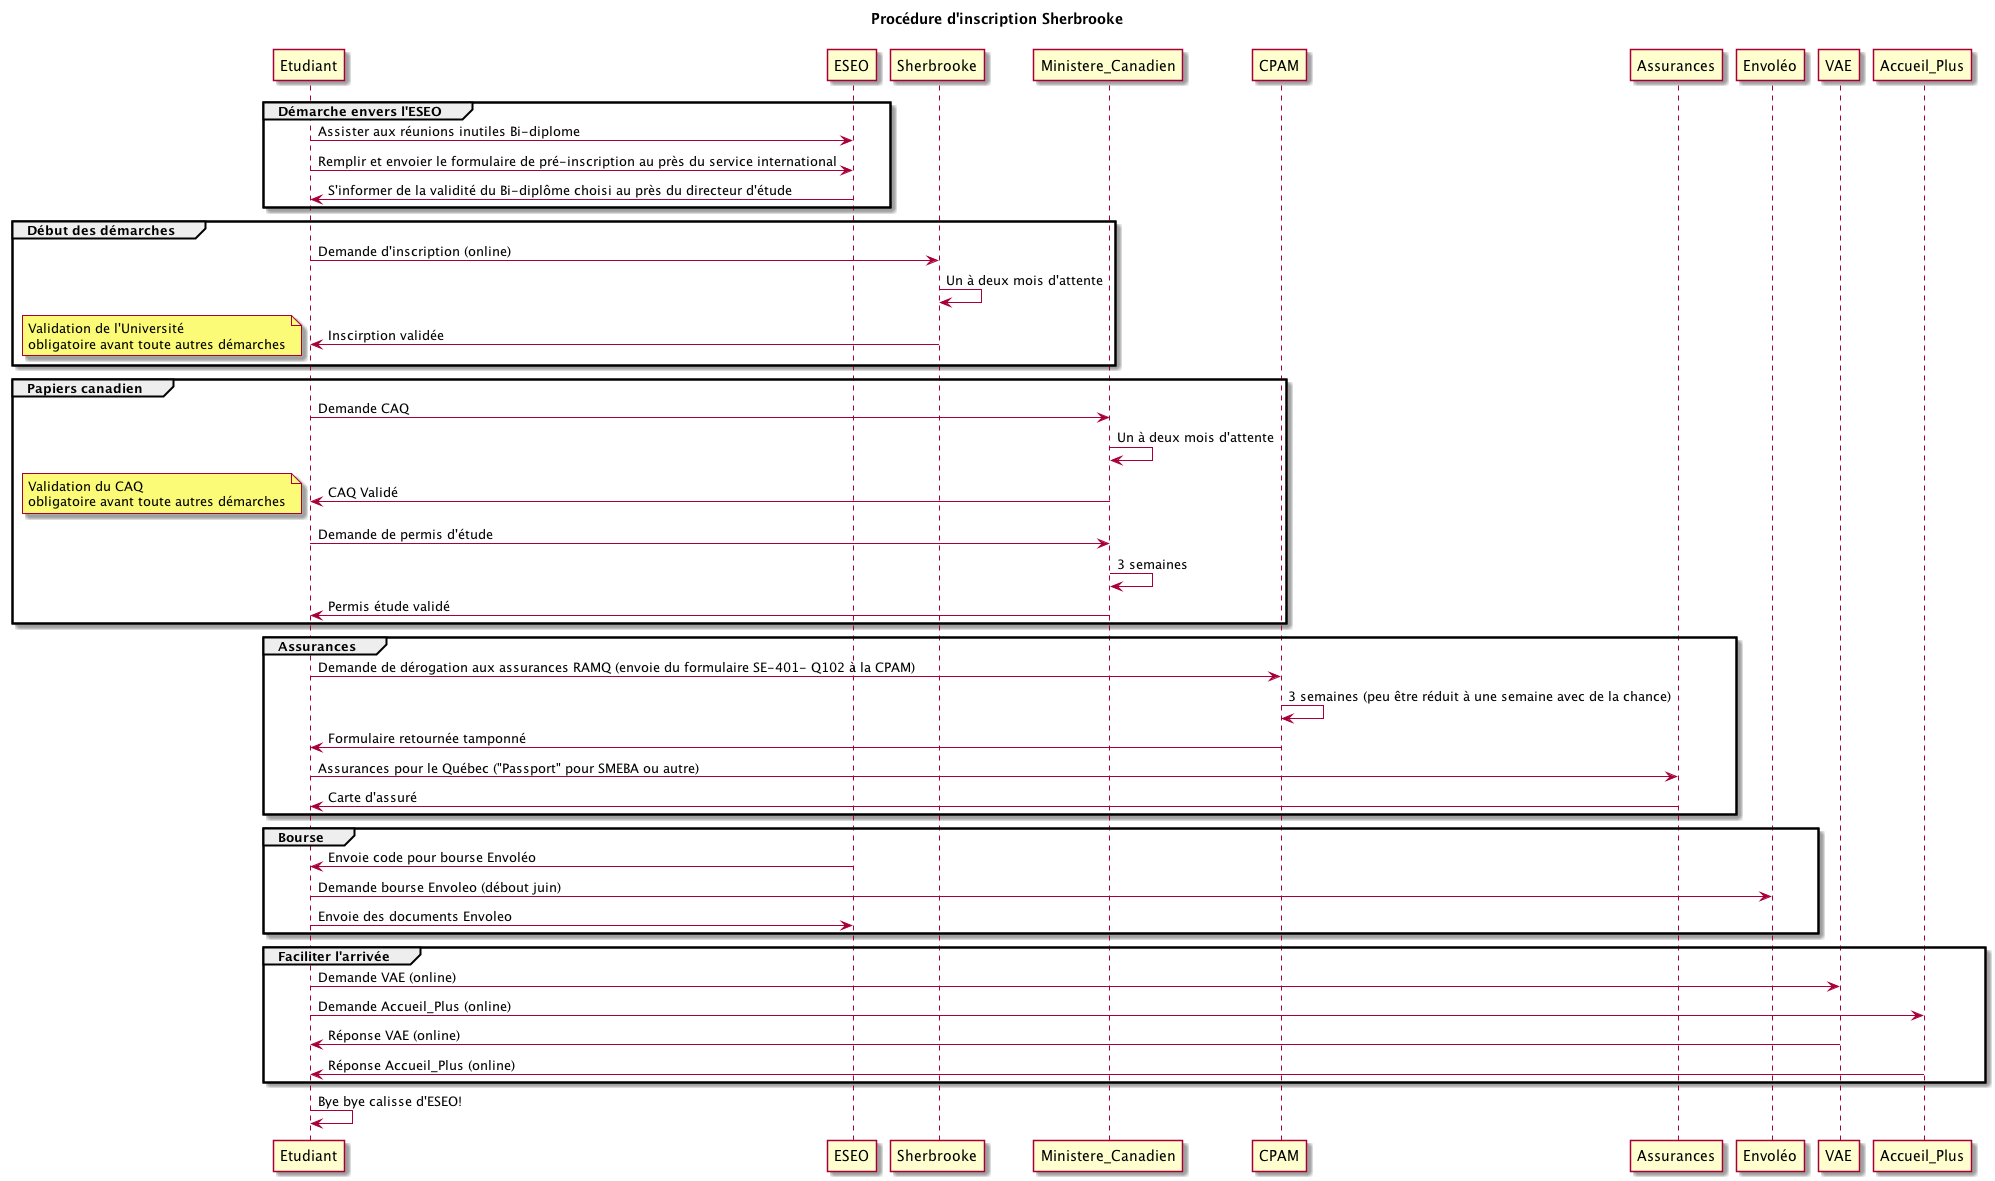
\includegraphics[width = 230mm, angle =90]{figures/Incri_Sherbrooke}
 \caption{Récapitulatif des actions a faire}
 \end{figure}
